This appendix contains a few examples of new drawing-artwork pairs found using the FT Aug and FT Aug Mini-Replica models. These pairs were not known earlier and were not part of the group of manually annotated pairs.

\begin{figure}
     \centering
     \begin{subfigure}[b]{0.45\textwidth}
         \centering
         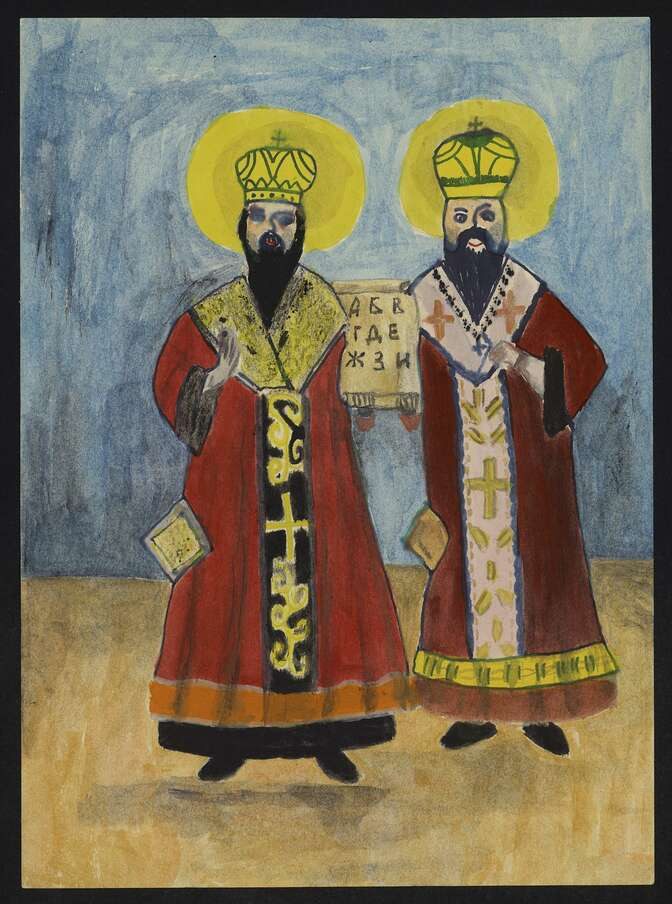
\includegraphics[width=\textwidth]{images/new_discoveries/2004_14-17_1013_BLG_R_C.jpg}
         \caption{Drawing: \texttt{2004\_14-17\_1013\_BLG\_R\_C}}
         \label{fig:2004_14-17_1013_BLG_R_C}
     \end{subfigure}
     \hfill
     \begin{subfigure}[b]{0.45\textwidth}
         \centering
         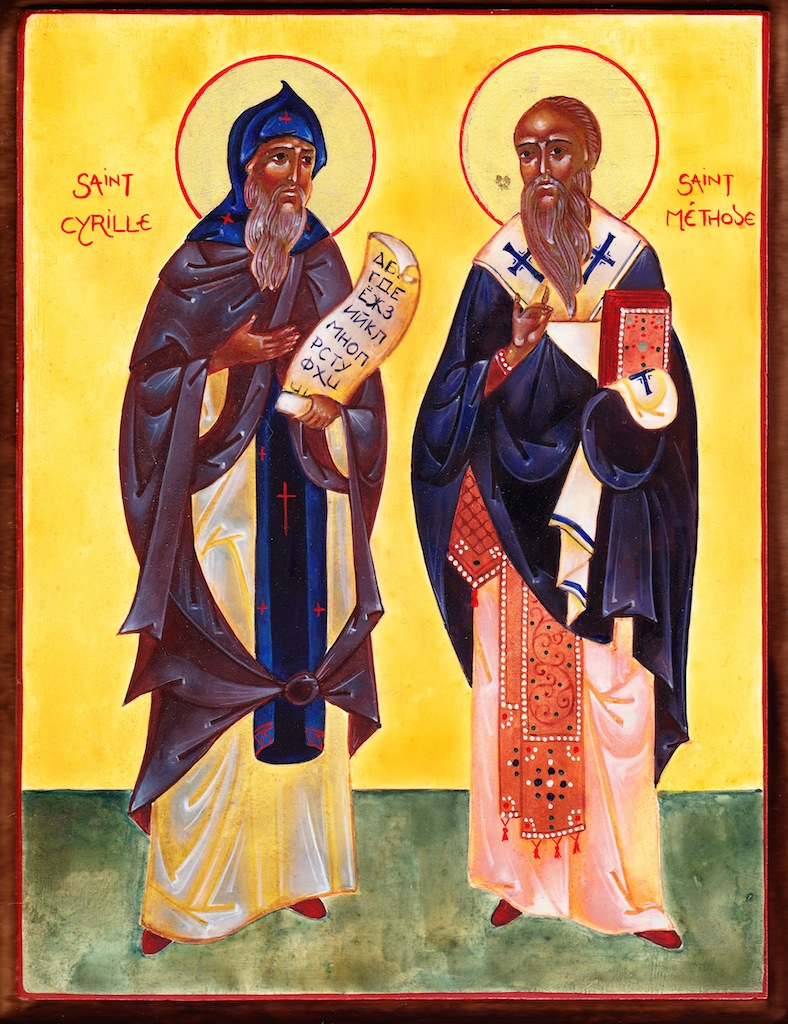
\includegraphics[width=\textwidth]{images/new_discoveries/cyrille-et-methode.jpg}
         \caption{Artwork: Cyril and Methodius}
         \label{fig:cyrille-et-methode}
     \end{subfigure}
     \caption{Discovered Drawing-Artwork Pair: 1}
\end{figure}

\begin{figure}
     \centering
     \begin{subfigure}[b]{0.45\textwidth}
         \centering
         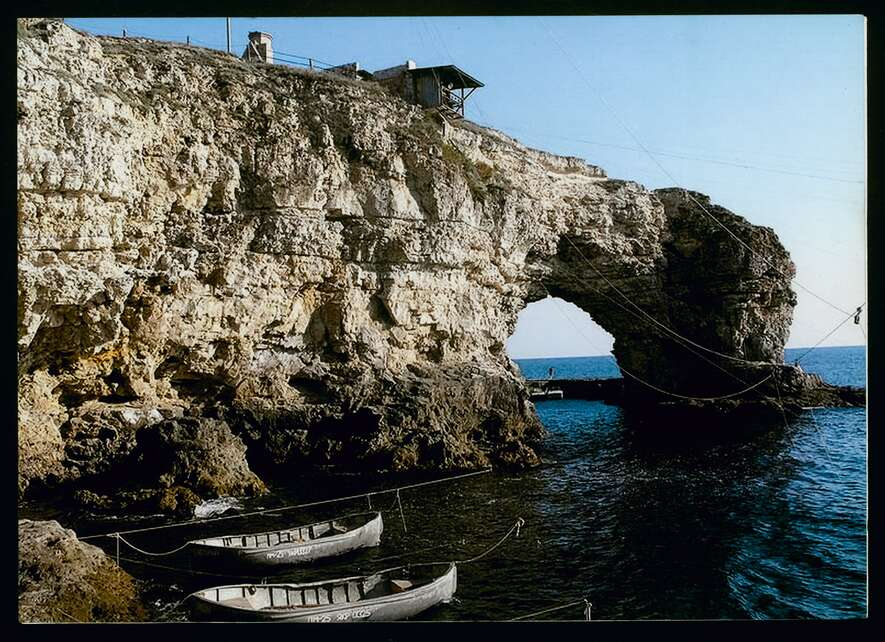
\includegraphics[width=\textwidth]{images/new_discoveries/2011_14-17_2059_UKR_R_C.jpg}
         \caption{Drawing: \texttt{2011\_14-17\_2059\_UKR\_R\_C}}
         \label{fig:2011_14-17_2059_UKR_R_C}
     \end{subfigure}
     \hfill
     \begin{subfigure}[b]{0.45\textwidth}
         \centering
         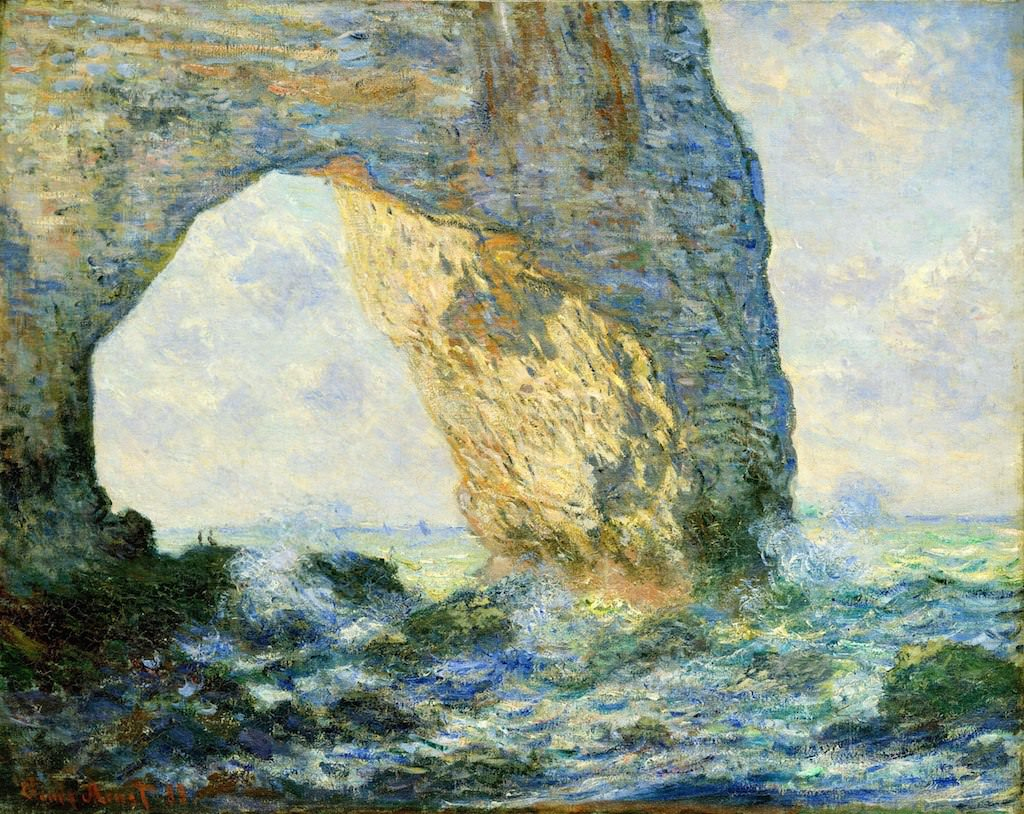
\includegraphics[width=\textwidth]{images/new_discoveries/Claude_Monet_23.jpg}
         \caption{Artwork: La Manneporte (Étretat) by Claude Monet}
         \label{fig:Claude_Monet_23}
     \end{subfigure}
     \caption{Discovered Drawing-Artwork Pair: 2}
\end{figure}


\begin{figure}
     \centering
     \begin{subfigure}[b]{0.45\textwidth}
         \centering
         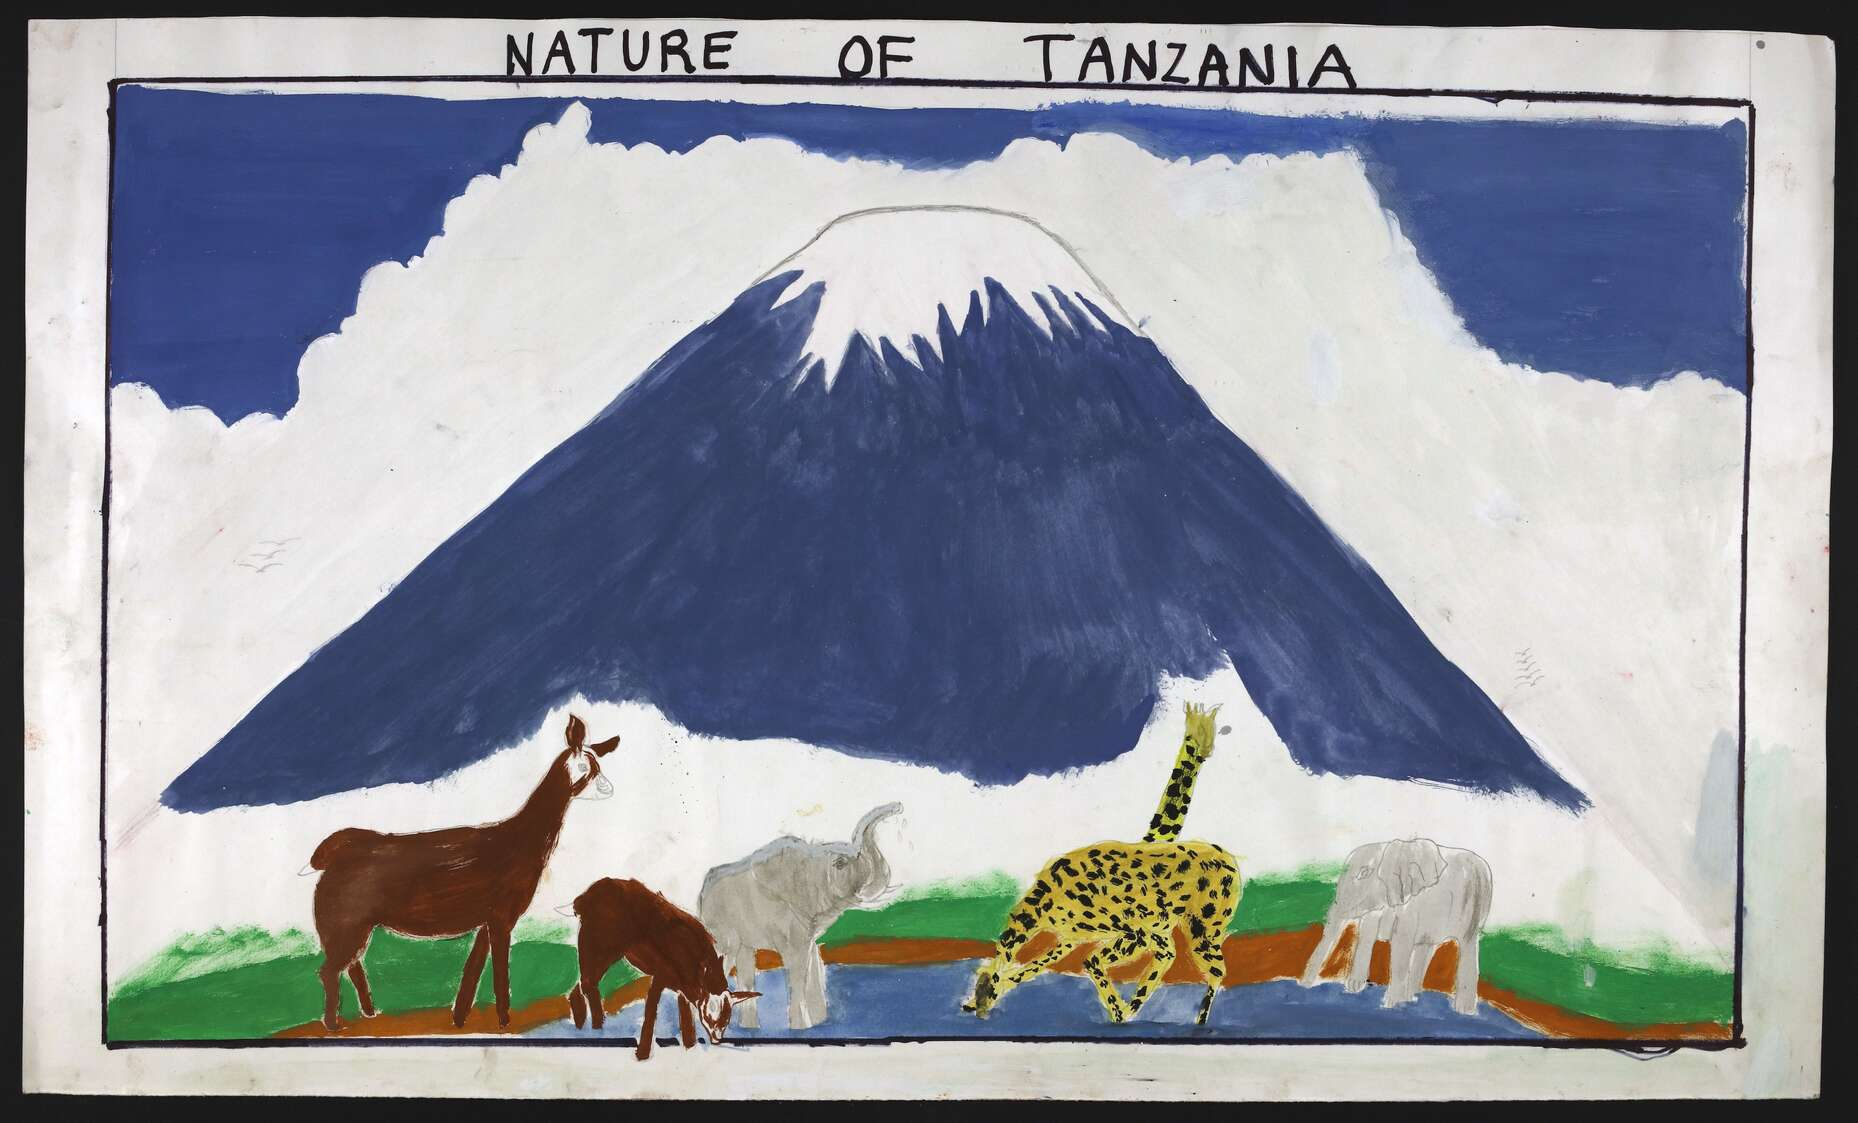
\includegraphics[width=\textwidth]{images/new_discoveries/1998_14-17_0441_TAN_R_C.jpg}
         \caption{Drawing: \texttt{1998\_14-17\_0441\_TAN\_R\_C}}
         \label{fig:1998_14-17_0441_TAN_R_C}
     \end{subfigure}
     \hfill
     \begin{subfigure}[b]{0.45\textwidth}
         \centering
         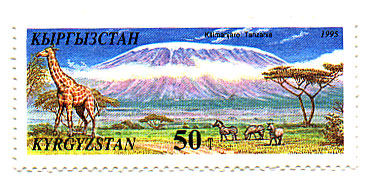
\includegraphics[width=\textwidth]{images/new_discoveries/kyrgyzstan_stamp_of_kilimanjaro.jpg}
         \caption{Artwork: A stamp of Mount Kilimanjaro}
         \label{fig:kyrgyzstan_stamp_of_kilimanjaro}
     \end{subfigure}
     \caption{Discovered Drawing-Artwork Pair: 3}
\end{figure}


\begin{figure}
     \centering
     \begin{subfigure}[b]{0.45\textwidth}
         \centering
         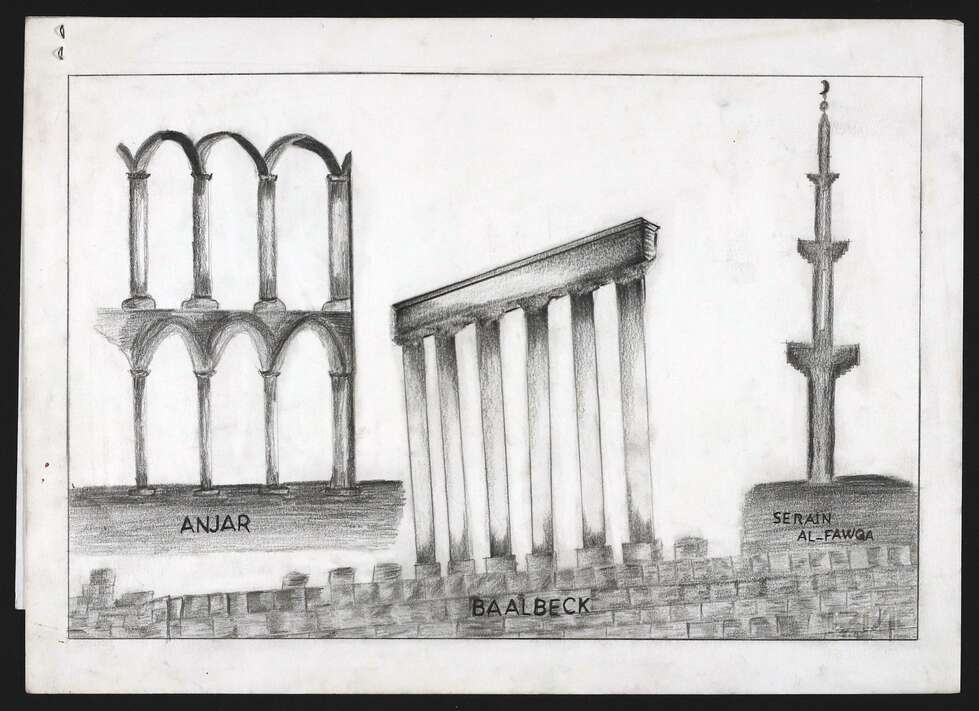
\includegraphics[width=0.5\textwidth]{images/new_discoveries/1998_18-25_0080_LBA_R_C.jpg}
         \caption{Drawing: \texttt{1998\_18-25\_0080\_LBA\_R\_C}}
         \label{fig:1998_18-25_0080_LBA_R_C}
         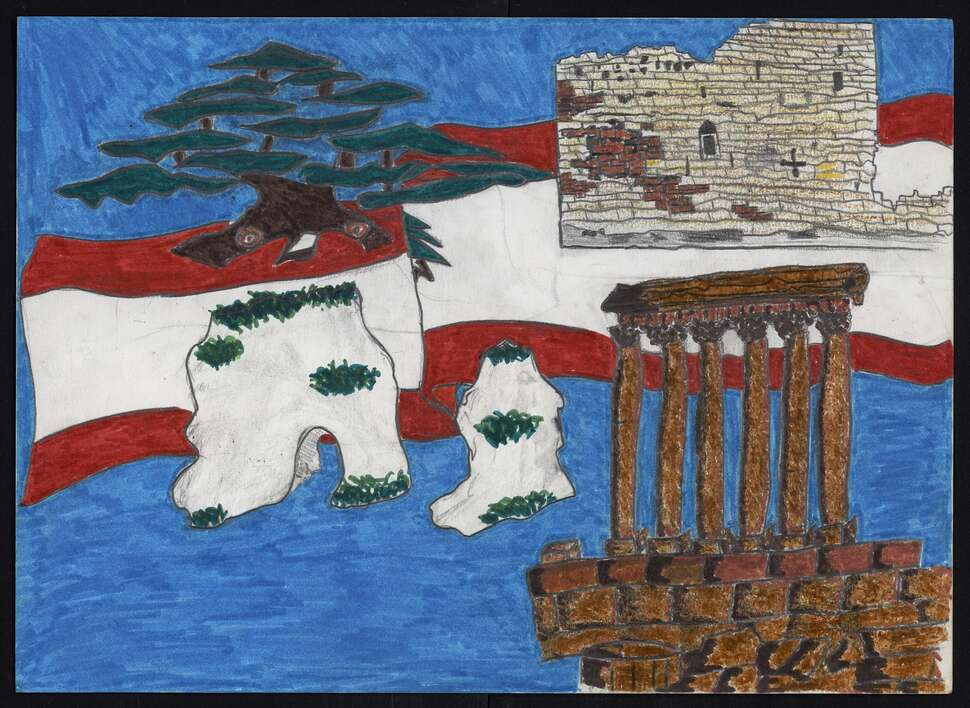
\includegraphics[width=0.5\textwidth]{images/new_discoveries/1998_14-17_0125_LBA_R_C.jpg}
         \caption{Drawing: \texttt{1998\_14-17\_0125\_LBA\_R\_C}}
         \label{fig:1998_14-17_0125_LBA_R_C}
     \end{subfigure}
     \hfill
     \begin{subfigure}[b]{0.45\textwidth}
         \centering
         \hfill
         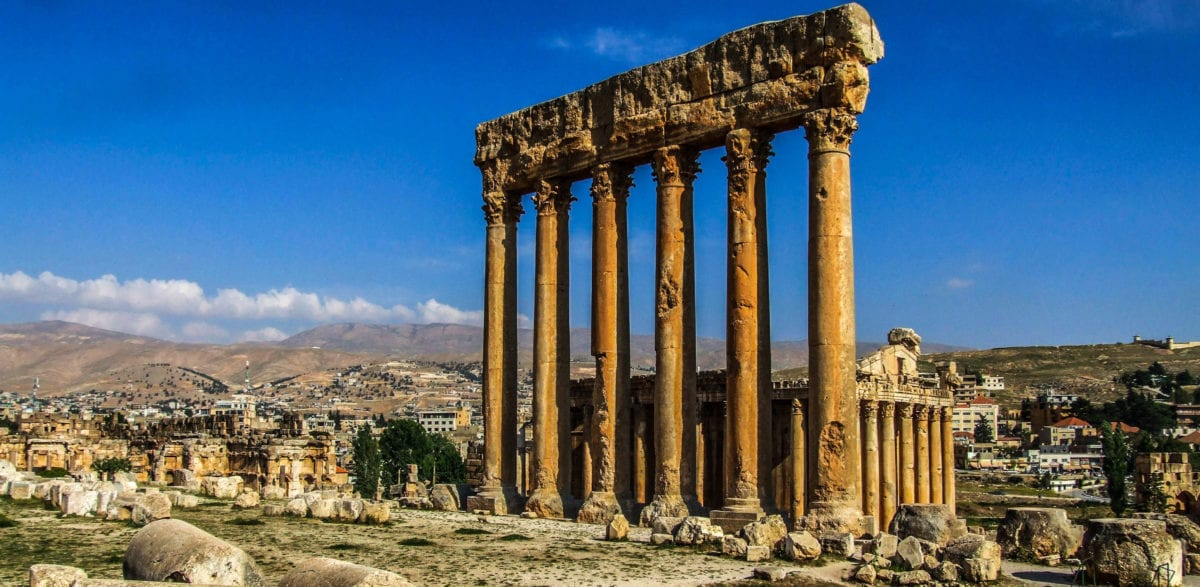
\includegraphics[width=\textwidth]{images/new_discoveries/baalbek_temple-of-jupiter.jpg}
         \hfill
         \caption{Artwork: Ruins of Temple of Jupiter in Baalbek, Lebanon}
         \label{fig:baalbek_temple-of-jupiter}
     \end{subfigure}
     \caption{Discovered Drawing-Artwork Pair: 4}
\end{figure}


\begin{figure}
     \centering
     \begin{subfigure}[b]{0.45\textwidth}
         \centering
         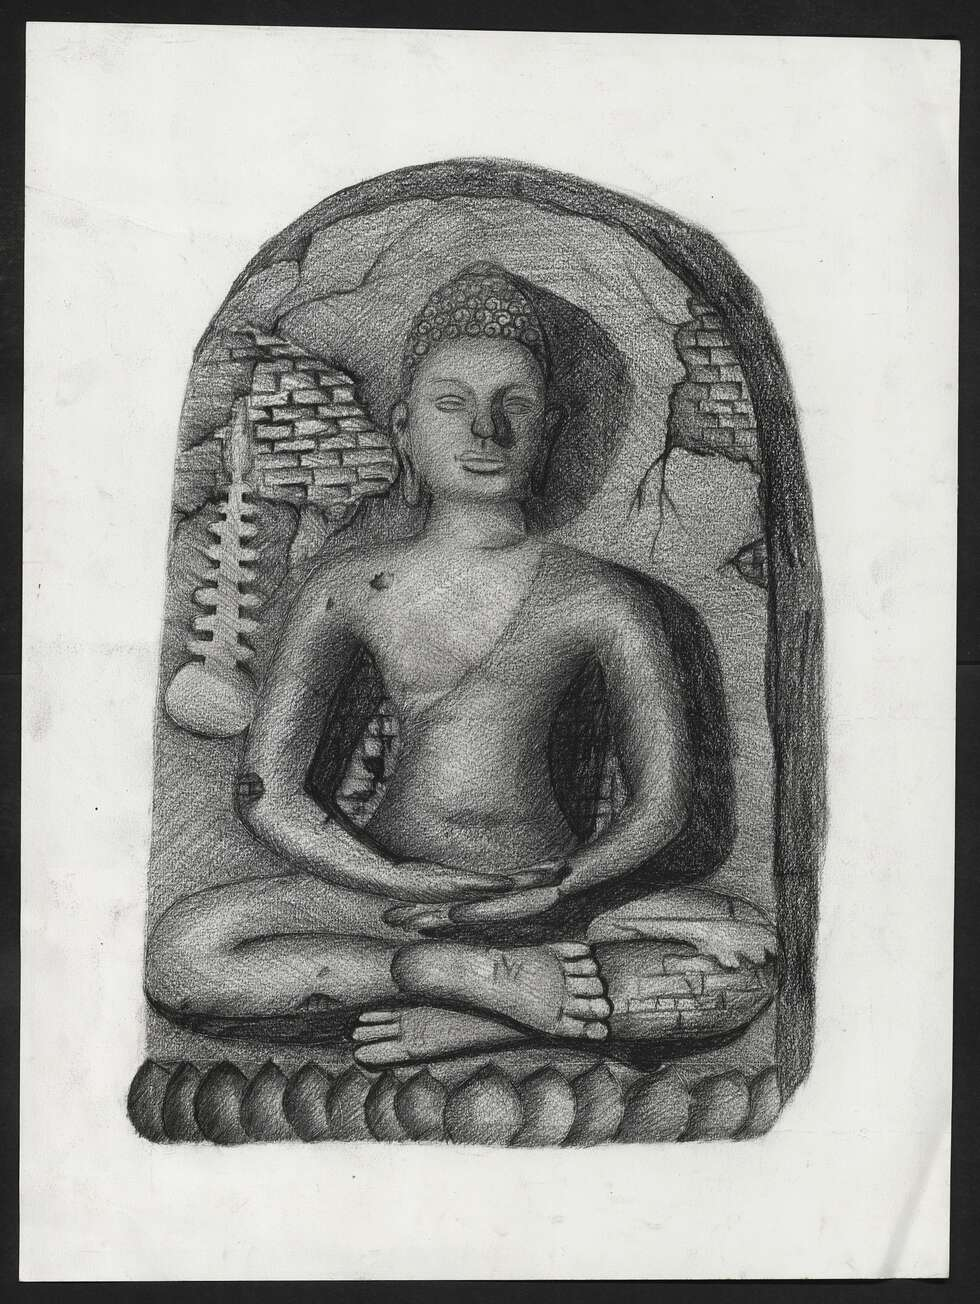
\includegraphics[width=\textwidth]{images/new_discoveries/2003_14-17_1243_THA_R_C.jpg}
         \caption{Drawing: \texttt{2003\_14-17\_1243\_THA\_R\_C}}
         \label{fig:2003_14-17_1243_THA_R_C}
        %  \includegraphics[width=0.6\textwidth]{images/new_discoveries/2004_14-17_0935_IMA_R_C.jpg}
        %  \caption{Drawing: \texttt{2004\_14-17\_0935\_IMA\_R\_C}}
        %  \label{fig:2004_14-17_0935_IMA_R_C}
     \end{subfigure}
     \hfill
     \begin{subfigure}[b]{0.45\textwidth}
         \centering
         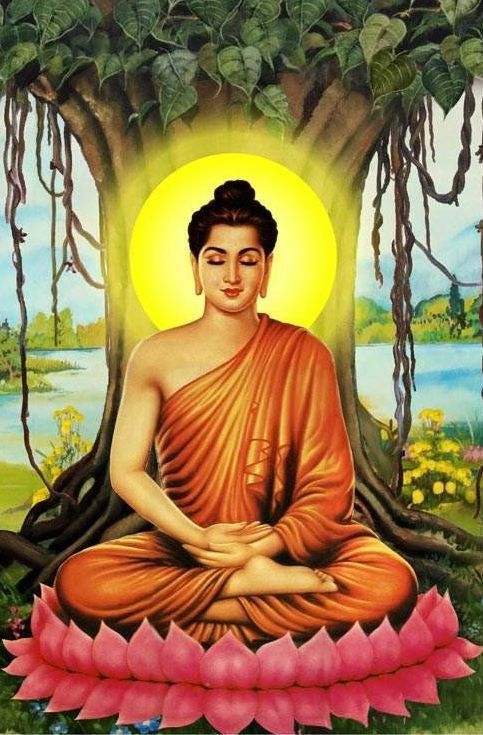
\includegraphics[width=\textwidth]{images/new_discoveries/buddha-eyes-closed.jpg}
         \caption{Artwork: Buddha sitting under a tree}
         \label{fig:buddha-eyes-closed}
     \end{subfigure}
     \caption{Discovered Drawing-Artwork Pair: 5}
\end{figure}
